\chapter{Thermal conductivity simulations of Silica glass}  \label{ch:silica}

The simulation of an amorphous system such as a-SiO$_2$ with classical MD and the estimation of its thermal conductivity require a few ingredients. 
First of all, we need a good interatomic force field that faithfully reproduces the structural and dynamical properties of the glass. Both will be important to correctly predict the thermal conductivity.
%and will be briefly discussed in Sec.~\ref{sec:silica-force-field}.
Second, we need to choose a system size and generate the amorphous structure, a process that is usually performed by melting and equilibrating the system at high temperatures, followed by a cooling phase in which it is gradually brought to the target temperature. At this point the system is equilibrated and data can start to be collected. This ``quenching'' protocol also affects the final structural and vibrational properties of the sample, hence we expect the thermal conductivity to be affected by its details. We shall introduce both these points in Section~\ref{sec:silica-classical} of this chapter. 

In Sec.~\ref{sec:results-class} we will present the method and the results of our classical simulations of vitreous silica using the ``BKS'' potential. The dependency of the computed thermal conductivity on many of the simulation parameters, such as sample size and quenching protocol, will be discussed.
Then, one \LEnote{*(a few)*} sample of silica will be chosen and its thermal conductivity studied as a function of the temperature. 

All this classical study will be instrumental in determining the feasibility of \abinitio calculations of thermal conductivity of a-SiO$_2$, using the DFT formulation of the heat flux that was presented in Chapter~\ref{ch:dft-heat}. One classical sample will be selected and simulated with Car-Parrinello MD at four different temperatures. The trajectory thus generated will be used to compute the \abinitio heat current and thermal conductivity using the GK equation, making use of many of the concepts and techniques discussed in Chapter~\ref{ch:data-analysis}. The simulation details and results will be presented in Sec.~\ref{sec:results-quantum}.


%%%%%%%%%%%%%%%%%%%%%%%%%%%%%%%%%%%%%%%%%%%%%%%%%%%%%%%%%%%%%%%%%%%%%%%%%
\section{Classical simulations of a-SiO$_2$}  \label{sec:silica-classical}

\subsection{BKS force field}  \label{sec:silica-force-field}

\LEnote{* FIGURA? *}

The structure of amorphous silica is made of SiO$_4$ tetrahedra, where silicon is at the center, bonded to 4 oxygen atoms located at the vertices. Each oxygen, in turn, bridges the tetrahedral corners, bonding between two silicon centers. The variation in orientation of adjacent tetrahedra makes the medium- and long-range structures disordered, forming a typical glass network.

One of the most successful and broadly adopted force fields for a-SiO$_2$ is the so-called BKS potential \cite{Silica-BKS-1990}. 
The BKS potential was devised by \citeauthor*{Silica-BKS-1990} who fitted self-consistent-field Hartree-Fock calculations on small silica clusters, and it is defined as the sum of a Coulomb and a Buckingham potential:
\begin{equation}
    v_{\alpha\beta}^{\mathrm{BKS}}(R) = q_\alpha q_\beta \mathtt{e}^2 V_C(R) + A_{\alpha\beta}\mathrm{e}^{-B_{\alpha\beta}R} - \frac{C_{\alpha\beta}}{R^6}, \label{eq:BKS}
\end{equation}
where $\alpha,\beta \in [\text{Si},\text{O}]$, and $R$ is the distance between the ions $\alpha$ and $\beta$. 

Despite its simplicity, BKS was showed to predict remarkably well many properties of SiO$_2$, among which its complicated phase diagram \cite{Saika2004}. 
Many other force fields have been used in the literature, ranging from simple two-body potentials like the BKS or re-parametrizations of it \cite{Carre2008}, to polarizable force fields (\emph{e.g.} \citet{Tangney2002}) and reactive ones (\emph{e.g.} ReaxFF \cite{Yuan2001}). 
Notwithstanding, the BKS potential is still the mostly adopted force field in classical simulations of a-SiO$_2$, thanks to its ability to reproduce very good glass structures. 
In the following, and partly in Sec.~\ref{sec:silica-quenching}, we are going to summarize how well the properties of amorphous silica are reproduced by this potential and others.


\paragraph{Structural properties}

Si-O bonds are generally considered to have partial ionic and covalent character. The BKS potential is spherical, therefore it does not describe the directional nature of the covalent bond, but it can anyway achieve the tetrahedral structure through a strictly repulsive interaction between oxygen atoms. We can expect that the bond's directionality could be better described by other more sophisticated potentials or by \abinitio methods, yet the BKS' abilities in predicting the amorphous structure of silica glass are very remarkable. 

For example, \citet{Tian2017} compared the structures of silica obtained from different force fields, \emph{e.g.} BKS and ReaxFF. They quenched a fully melted silica box of density $\rho=2.2\un{g/cm^3}$ from $5000\un{K}$ to $300\un{K}$ at $5\times 10^{12}\un{K/s}$ in the NVT ensemble. 
The BKS and ReaxFF potentials both generate realistic silica structures \cite{Vollmayr1996,Yuan2001}, with radial distribution functions, neutron structure factors, and coordination numbers that reasonably reproduce the experimental observations.
The radial distribution functions, in very good agreement with experiment, show a sharp peak correspondent to the Si-O bond length at $\sim 1.6\un{\angstrom}$, the peak correspondent to the O-O distance at $\sim 2.6\un{\angstrom}$, and the one correspondent to the Si-Si distance at $\sim 3.1\un{angstrom}$. 

The coordination numbers can be used to detect coordination defects. By choosing a cutoff length for Si-O pairs of $\sim 2.15\un{\angstrom}$, BKS reproduces a realistic coordination environment for Si and O, with over $99.6\%$ of atoms being normally coordinated (4-fold Si and 2-fold O). ReaxFF, instead, tends to generate more coordination defects, with $\sim 97.5\%$ of normally coordinated atoms.
Nevertheless, the quenching process largely influences the macroscopic and microscopic properties of the generated glass, so we shall comment more on these point later, in Sec.~\ref{sec:silica-quenching}. 


\paragraph{Vibrational properties}

\begin{figure}[!tb]
    \centering
    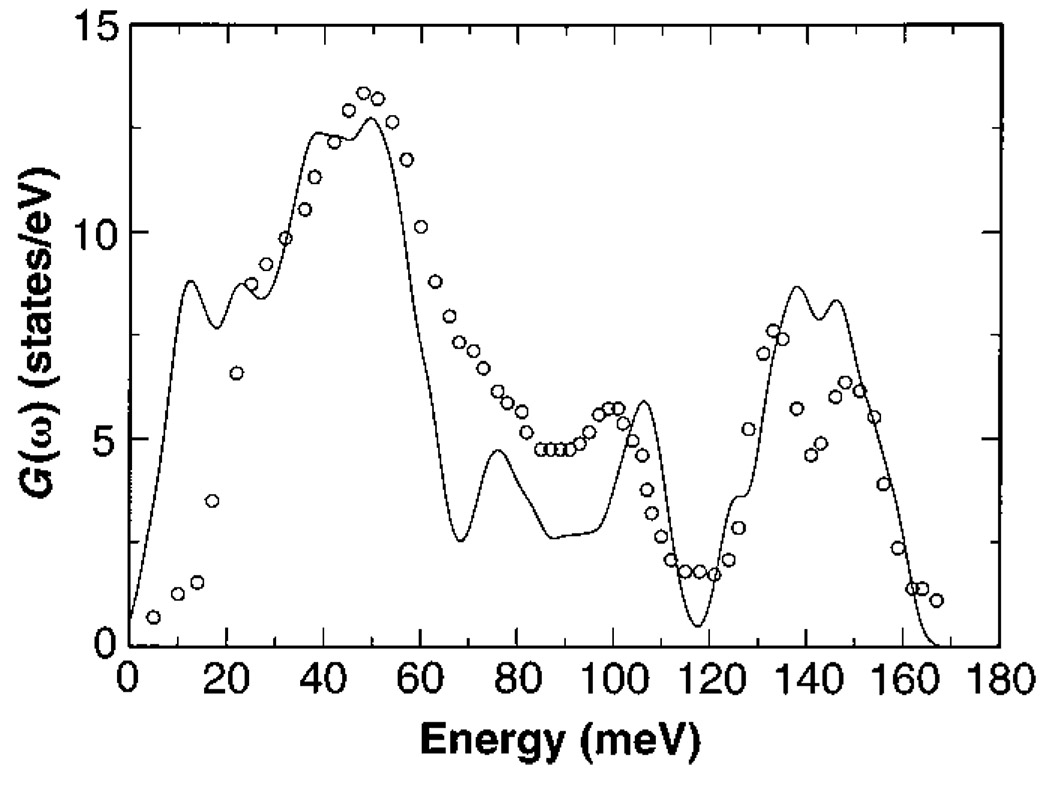
\includegraphics[width=8cm]{chapters/chapter6/figures/Sarnthein_Car_abinitio_VDOS_silica-2.jpg}
    \caption{
    Effective vibrational density of states of an a-SiO$_2$ sample of $72$ atoms at experimental density $2.20\un{g/cm^3}$, computed from AI-CPMD simulations within the local density approximation (solid line), compared to neutron scattering data (circles). Reproduced from Ref.~\cite{Sarnthein1997}.}
    \label{fig:silica-vdos-abinitio}
\end{figure}
\begin{figure}[!tb]
    \centering
    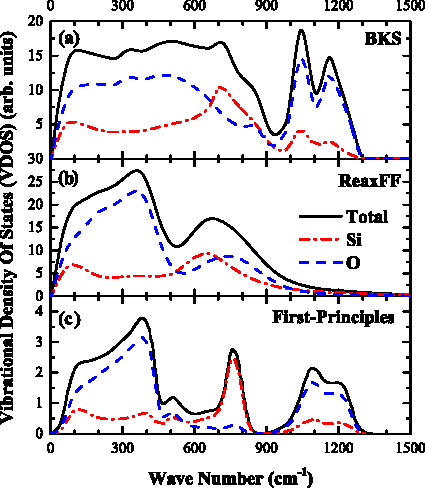
\includegraphics{chapters/chapter6/figures/Tian_VDOS_silica.pdf}
    \caption{
    Total and partial VDOS of a-SiO$_2$ computed for the (a) BKS and (b) ReaxFF, and compared with the (c) first-principles results of \citet{Bhattarai2016}. Adapted from Ref.~\cite{Tian2017}.}
    \label{fig:silica-vdos-classical}
\end{figure}

Besides the structure of the generated sample, what determine the thermal conductivity of the system are its vibrational properties, that are determined by the interaction potential and can be analyzed by the vibrational density of states (VDOS).
Experimentally, the VDOS obtained from neutron scattering shows three significant peaks at about $400$, $800$, and $1100\un{cm^{-1}}$, that represent the rocking, bending, and stretching modes respectively \cite{Galeener1983}, as shown in Fig.~\ref{fig:silica-vdos-abinitio}.

First principles simulations have shown to successfully reproduce all the principle peaks of the VDOS. \citet{Sarnthein1997} studied a sample of $72$ atoms of a-SiO$_2$ obtained by a quench from the melt with AIMD at experimental density ($2.20\un{g/cm^3}$), within the local density approximation of DFT, and computed the VDOS by diagonalization of the dynamical matrix. Their results, reported in Fig.~\ref{fig:silica-vdos-abinitio}, are in very good agreement with the experiments. The same calculation has been reproduced more recently by \citet{Bhattarai2016} using a $648$-atom model of a-SiO$_2$ (see Fig.~\ref{fig:silica-vdos-classical}). 

Conversely, classical force fields struggle to correctly reproduce the features of the VDOS of a-SiO$_2$. In Fig.~\ref{fig:silica-vdos-classical} we report the VDOS obtained for the BKS and ReaxFF potentials \cite{Tian2017}, compared to \abinitio calculations \cite{Bhattarai2016}. 
The low-frequency band is dominated by O contributions and agrees well with the results of first-principles simulations and experiments, even though it wrongly elongates up to $600\un{cm^{-1}}$ using the BKS potential. For this model, the modes in the $400-500\un{cm^{-1}}$ range do not agree well with experiment, a sign suggesting that BKS struggles to reproduce correctly the forces over intermediate-range distances \cite{Vollmayr1996,Benoit2002}. 
The intermediate-frequency band of \abinitio simulations is dominated by Si contributions and presents an isolated peak at about $800\un{cm^{-1}}$, but this is not reproduced by the BKS potential, while ReaxFF does not account correctly for the contributions of Si and O atoms. 
The high-frequency band, that corresponds to Si-O stretching vibrations, is well reproduced by the BKS potential, but is notably missing in ReaxFF. 

The vibrational excitations of silica include very localized modes and collective ones (most modes with frequencies below $22\un{THz}$ have a collective nature, while the ones at higher frequencies are more localized). Compared to the \abinitio description, the BKS does not reproduce well the nature of modes in the intermediate frequency range \cite{Benoit2002}. Since the BKS model was designed to optimize the elastic constants of a small silica cluster and a crystal, it is not very surprising that it performs well at very high and low frequencies, but it is not reliable at intermediate frequencies. 

Therefore we can expect that ReaxFF will provide more realistic predictions of thermal conductivity at room temperature, where thermal conduction is mainly contributed by acoustic-like phonon vibrations whose frequencies are typically below $400\un{cm^{-1}}$ \cite{Bhattarai2016}; whereas the BKS potential will probably be more suitable to study high-temperatures cases, where the contribution of stretching vibrations to thermal conduction increases significantly \cite{Tian2017}. 



\subsection{Sample size and preparation}  \label{sec:silica-size}
In contrast to crystals, glasses have a completely disordered and non-periodic structure, therefore we should understand what is the minimum sample size that one should simulate to ensure that the distribution of structures is well represented. This is of particular importance in view of performing AIMD simulations, in which the computationally affordable sizes are of the order of a few hundreds of atoms at most. Previous studies have tried to survey this limit. 

Few studies have been performed using \abinitio techniques and all involved a small sample of $\sim 70$ atoms ($\sim 25$ SiO$_2$ units). In the first \abinitio simulation of a-SiO$_2$, \citet{Sarnthein1995a} performed a quench from the melt completely by CPMD, obtaining a first model of vitreous silica. Even though good agreement with experiments was found for some structural, vibrational and electronic properties \cite{Sarnthein1995a,Sarnthein1995b,Sarnthein1997}, a very fast quenching rate (of the order of $10^{15}\un{K/s}$) was used, due to the high computational cost, that may have strongly influenced the results. In Sec.~\ref{sec:silica-quenching} we will debate more this issue. 
Some years later, \citet{Benoit2000} combined classical MD with CPMD: samples generated with the BKS potential (with a quenching rate $\sim 10^{13}\un{K/s}$) were then equilibrated in CPMD. It was shown that the structural properties thus obtained were weakly modified with respect to the classical calculations, thus validating the structural model generated with the BKS potential. Besides, these results were even in better agreement with experiments with respect to previous studies performed completely in CPMD, which is probably due to the slower quenching employed. 
Other five years later, \citet{VanGinhoven2005} studied a set of small silica samples of $72$ atoms generated by the BKS potential and optimized by DFT, and showed that by creating multiple small samples it is possible to achieve a good statistical sampling of structural features consistent with larger simulated glass systems. An ensemble of small samples is necessary to capture the statistical distribution of structures of silica glass, \emph{i.e.} all the possible arrangements of its medium range structures. 

In spite of the reliability of BKS with regard to structural properties, as mentioned in the previous Section, the vibrational properties reproduced by this classical force field are strongly modified by using an \abinitio treatment of the forces \cite{Benoit2002}, therefore we do not expect it to be reliable in this respect. 
Furthermore, it is not yet clear how much the thermal conductivity is affected by the size of the sample. Even if we average over a set of small samples, it is possible that $\kappa$ intrinsically requires larger size cells to converge. Finite-size effects, due to PBC, may be relevant and influence the computed $\kappa$. 
Therefore, a preliminary study on this point should be performed before attempting an \abinitio computation of the thermal conductivity of a-SiO$_2$. We will present the results of this study in Sec.~\ref{sec:results-class-quench}.



\subsection{Quenching}  \label{sec:silica-quenching}

The properties of the simulated glass may sensibly depend on the quenching protocol adopted to generate the virtual sample. 
When a supercooled liquid is cooled down so much that the relaxation times of the system exceed the time scale of the (virtual) experiment, the system will be in a nonequilibrium state and undergo a glass transition, provided it does not crystallize. The obtained glass is a nonequilibrium structure whose properties will generally depend on its production history. The \emph{quenching rate} at which it was cooled will determine its macroscopic and, in particular, microscopic properties \cite{Vollmayr1996}. 
For example, the glass transition temperature computed by simulations is significantly higher than the glass transition temperature observed in the laboratory. 
The time scales reachable by computer simulations are many orders of magnitude shorter than the typical time scales of laboratory experiments, hence the minimum quenching rates attainable in classical MD simulations are of the order of $10^{11}-10^{13}\un{K/s}$, a rate that can only be replicated experimentally by strong laser pulses or ion bombardment \cite{Soules2011}.


\paragraph{Macroscopic properties}
\citet{Vollmayr1996} extensively studied the effects of quenching rate on the properties of BKS amorphous silica. They used a sample of $\sim 1000$ atoms at zero pressure, melted at $7000\un{K}$ and then cooled down to $0\un{K}$ at different temperature rates $\gamma$, ranging from $10^{12}$ to $10^{15}\un{K/s}$. More recently, \citet{Lane2015} extended their study, reaching cooling rates down to $5\times 10^{9}\un{K/s}$ with microsecond MD simulations of $\sim 13000$ atoms.

\begin{figure}[!tb]
    \centering
    \subfigure[\label{fig:silica-bks-density-anomaly}]{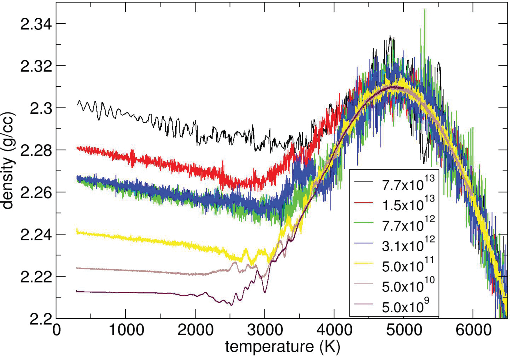
\includegraphics[height=4.6cm]{chapters/chapter6/figures/Lane_density1.pdf}}
    \hfill
    \subfigure[\label{fig:silica-bks-density-temp}]{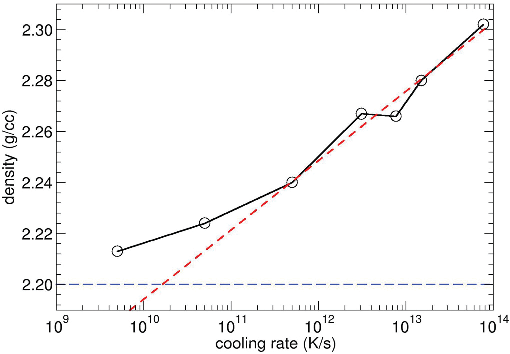
\includegraphics[height=4.6cm]{chapters/chapter6/figures/Lane_density2.pdf}}
    \caption{
    (a) Density vs temperature of a-SiO$_2$, modelled with the BKS potential, for seven quenches completed with linear cooling rates $\gamma$ from $8000\un{K}$ to $300\un{K}$. Silica's density anomaly is visible at high temperatures; density becomes independent of $\gamma$ at $T \gtrsim 4500\un{K}$. 
    (b) Density at $300\un{K}$ as a function of the quench cooling rate $\gamma$. The horizontal dashed line is the experimental value. The red dashed line is a linear extrapolation fit to data above $3\times 10^{12}\un{K/s}$. 
    Reproduced from Ref.~\cite{Lane2015}}
    \label{fig:silica-bks-density}
\end{figure}

The glass transition temperature, that they estimated from the enthalpy curves, increases with $\gamma$. As one can expect, fast cooling rates make the system fall out of equilibrium more quickly during the quench. 
The density $\rho$ of the final sample also depends on the quenching rate: at temperatures below $2000-3000\un{K}$, higher $\gamma$ determine higher densities, as can be observed in Fig.~\ref{fig:silica-bks-density}, that seem to approach the experimental value of $2.202\un{g/cm^3}$. Between $10^{14}\un{K/s}$ and $10^{9}\un{K/s}$ density decreases of less than $5\%$. 
This behavior is unusual: in most glasses density increases as cooling rates are slowed. \LEnote{**CHECK**} It can be explained by observing the trend at higher temperatures, where the density reaches a maximum at $T\sim 4800\un{K}$ that does not depend on $\gamma$: this ``density anomaly'' is also observed in experiments, at a much lower temperature of $1820\un{K}$. This discrepancy can be attributed to the BKS potential \LEnote{and to the finite size of the simulation domain.}  
Furthermore, the thermal expansion coefficient at constant pressure, $\alpha_p = \frac{1}{V} \left.\frac{\partial V}{\partial T}\right|_p = -\frac{1}{\rho} \left.\frac{\partial \rho}{\partial T}\right|_p$, increases with $\gamma$.

\paragraph{Microscopic properties}
Microscopic properties are even more affected by the quenching rate. 
By analysing the radial distribution function (RDF) between different species it is possible to observe that a small cooling rate makes the structural order at short and intermediate distances increase, \emph{i.e.} the RDF peaks and minima are sharpened and the structure is more relaxed. However, the location of the RDF's peaks is very little affected by $\gamma$ (\emph{i.e.} the Si-O tetrahedra do not change much their size with $\gamma$) and compares quite well with experiment, thus making BKS a good potential to reproduce the short- and medium-range structure of a-SiO$_2$. 
The study of coordination numbers of each atom type shows that local order increases fast with decreasing cooling rate: for example, the number of Si atoms that are 4-fold coordinated with oxygen atoms increases from $95\%$ to $99.5\%$ by decreasing the cooling rate from $10^{15}\un{K/s}$ to $10^{13}\un{K/s}$, and even further at $10^{10}\un{K/s}$.
Since the size of Si-O tetrahedra does not change much their size with $\gamma$, the variation of density with the changes in the cooling rate is due to relative arrangement of neighboring tetrahedra. 
This can be observed in variations of the distributions of angles and rings. The O-Si-O angle distribution sharpens by decreasing $\gamma$ and approaches the ideal tetrahedron angle of $109.47^\circ$; the Si-O-Si angle distribution, instead, does not sharpen but shifts to larger angle values, indicating a more open arrangement of tetrahedra, which is consistent with the observed lower density; rings of size $6$ becomes more frequent with decreasing $\gamma$, indicating that the local structure of the system approaches the one of $\beta$-crystobalite. 
Finally, the two high-frequency peaks of VDOS depend on the quench rate in that their height increases significantly by decreasing $\gamma$, hence improving the agreement with experiment. 
The low- and mid-frequency bands obtained with the BKS, are quite featureless and do not change very much with $\gamma$, thus remaining quite in discordance with experimental results. 

In conclusion, even though these studies have been performed using the BKS potential and not with DFT (for obvious computational reasons), it is very reasonable to assume their results will also hold for AIMD simulations of amorphous silica. 
The demonstrated structure predictions capabilities of the BKS potential and the very large range of time scales analyzed leads us to conclude that a reliable a-SiO$_2$ structure can only be obtained by a ``slow'' quenching protocol with classical MD. 
However, to our knowledge a study of the dependence of thermal conductivity of a-SiO$_2$ on the quenching rate has never been attempted, and should be performed attempting a first-principles calculation. In Sec.~\ref{sec:results-class-quench} we will present this study. 



\subsection{Thermal conductivity: previous studies}  \label{sec:silica-kappa-studies}
\paragraph{Non-Equilibrium MD studies}
Many studies of the thermal conductivity of a-SiO$_2$ are based on NEMD simulations, that are strongly size dependent due to scattering of phonons with the heat sink, and thus require the study of its convergence at large cell sizes. 
For example, \citet{Tian2017} simulated a-SiO$_2$ with the BKS potential at $T=300\un{K}$, $\rho=2.2\un{g/cm^3}$, and obtained a value of thermal conductivity of $\kappa=(2.27 \pm 0.06)\un{W/mK}$ at the maximum size simulated, whereas \citet{Coquil2011} obtained $\kappa= (2.10 \pm 0.10)\un{W/mK}$. 

An extrapolation technique is needed to estimate the convergence of $\kappa$ as a function of the length of the simulation cell in the direction of the applied heat flux (or temperature gradient), $L_z$. According to the kinetic theory: $\kappa = \frac{1}{3} c_v v \,l$, where $c_v$ is the lattice specific heat at constant volume, $v$ is the sound velocity, and $l$ is the mean-free path of the phonons. The thermal conductivity can be obtained by linear fitting $1/\kappa$ vs $1/L_z$ and extrapolating the value at $1/L_z=0$ \cite{Schelling2002}. 
Despite being broadly applied in the literature, this method has to be used with extreme care. Indeed, if the distribution of phonon mean-free paths cannot be approximated by its average value, the linear dependence of $1/\kappa$ on $1/L_z$ is no longer valid, as higher-order terms are not negligible, as \citet{Sellan2010} ascertained studying Ar and Si crystals. If the considered system sizes are smaller than the largest bulk mean-free paths that dominate the thermal transport, then the linear relationship may not work and the thermal conductivity can be severely underestimated.

In the case of amorphous silica, the maximum phonon mean-free path is quite short ($\sim 6\un{\angstrom}$ \cite{Yu2006}), a fact that may explain why \citet{Tian2017} find the linear fit to work well in this case, allowing them to extrapolate a value of $\kappa=2.5\un{W/mK}$ for the BKS and Teter potentials, and of $1.28\un{W/mK}$ for the ReaxFF potential, at $300\un{K}$. Therefore, the ReaxFF potential seems to best reproduce the experimental value of $\kappa_{exp}\approx 1.3-1.4\un{W/mK}$ at this temperature. 


\paragraph{Equilibrium MD studies}
\LEnote{**PARAGRAFO DA RIVEDERE. Devo guardare questo articolo**}
Few studies have been performed using EMD, probably due to the difficulty in estimating the thermal conductivity from the GK equation, as we already described in Sec.~\ref{sec:data-analysis-methods}.
\citet{McGaughey2004b} was estimated the thermal conductivity of a system of $576$ atoms (\LE{$\rho=***$ at $T\sim \un{K}$}), obtaining a thermal conductivity of $1.96\un{W/mK}$. 
The GK method is much less affected by finite-size effets, and can simulate the bulk with much smaller systems, actually much smaller than the estimated phonon mean-free path \cite{Schelling2002}. As already mentioned in Sec.~\ref{sec:spectral-methods}, the potential finite-size effects of the GK method may be attributed to memory effects, \emph{i.e.} to phonons that, thanks to PBC, reenter the simulation box several times without scattering and hence may introduce artificial correlations. In this case, the heat flux autocorrelation function may not be reliable for times longer than the time required for the passage of the phonon across the simulation cell. 
\LE{**celle usate da McGaughey??**}
Tests for the convergence of $\kappa$ with the cell size should always be performed, and will be carried out for a-SiO$_2$ in Sec.~\ref{sec:results-class}.


\paragraph{Lattice methods????}
\LEnote{******ANYTHING***??}



%%%%%%%%%%%%%%%%%%%%%%%%%%%%%%%%%%%%%%%%%%%%%%%%%%%%%%%%%%
\section{Classical simulations: Results}  \label{sec:results-class}

\begin{figure}[!tb]
    \centering
    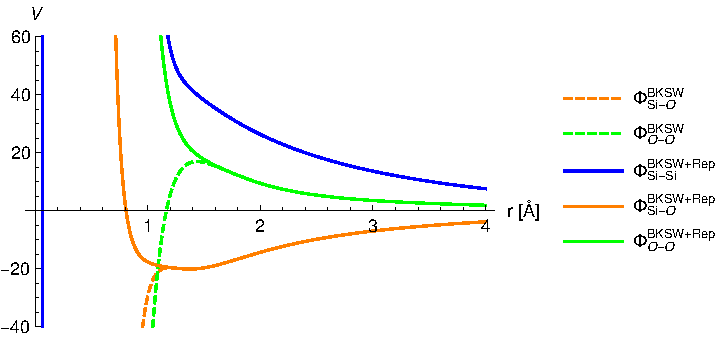
\includegraphics[]{chapters/chapter6/figures/BKSW.pdf}
    \caption{Dashed lines: BKS potential with Wolf truncation, as defined in Eq.~\eqref{eq:BKS-Wolf}. Solid lines: the same with a repulsive core added, defined in Eq.~\eqref{eq:BKS-repulsive-core}.}
    \label{fig:BKS-potential}
\end{figure}

We performed classical MD simulations of amorphous silica using the \textsc{LAMMPS} package \cite{LAMMPS1995}. 
We used a modified version of the BKS potential \cite{Carre2008}, in which the long-range Coulomb interaction is truncated with the Wolf method \cite{Wolf1992,Wolf1999,Fennel2006}, thus avoiding the use of Ewald summations \cite{Allen1989,Frenkel2001}. This truncation is possible thanks to Coulomb screening effects, and it only needs the addition of a correction term that recovers the requirement of charge neutrality. 
The final form we used is the one of Ref.~\cite{Mantisi2012}:
\begin{multline}
    v_{\alpha\beta}^{\mathrm{BKS}}(R) = q_\alpha q_\beta \mathtt{e}^2 V_W(R) G_W(R) + \\
    \left[ A_{\alpha\beta} \mathrm{e}^{-\frac{R}{\rho_{\alpha\beta}}} - \frac{C_{\alpha\beta}}{R^6} - \left( A_{\alpha\beta} \mathrm{e}^{-\frac{R_{c,\mathrm{sh}}}{\rho_{\alpha\beta}}} - \frac{C_{\alpha\beta}}{R_{c,\mathrm{sh}}^6} \right) \right] G_{\mathrm{sh}}(R) , \label{eq:BKS-Wolf}
\end{multline}
with
\begin{equation}
    v_W(R) = \left(\frac{1}{R}-\frac{1}{R_c}\right) + \frac{1}{R_c^2}\left(R-R_c\right) ,
\end{equation}
\begin{equation}
    G_W(R) = \exp \left( -\frac{\gamma_W^2}{(R-R_{c,W})^2} \right) , \quad
    G_{\mathrm{sh}}(R) = \exp \left( -\frac{\gamma_{\mathrm{sh}}^2}{(R-R_{c,\mathrm{sh}})^2} \right) ,
\end{equation}
$q_{\mathrm{Si}}=2.4$, $q_{\mathrm{O}}=-1.2$, $\gamma_W = \gamma_{\mathrm{sh}} = 0.5$, $R_{c,W} = 10.17\un{\angstrom}$, and $R_{c,\mathrm{sh}} = 5.5 \un{\angstrom}$.
This potential, whose form is depicted in Fig.~\ref{fig:BKS-potential}, was shown to give results comparable to the original BKS formula \cite{Carre2008}. 
Since the potential becomes attractive at very short distances, its short-range part at $R < R_{\mathrm{inf}}$ has been substituted by a repulsive core, in order to avoid atoms to get too close to each other: a problem that may arise at high temperatures during melting. The form of this repulsive part is:
\begin{equation}
    V_{\alpha\beta}^{\mathrm{rep}}(R < R_{\mathrm{inf}}) = \frac{D_{\alpha\beta}}{R^{12}} + E_{\alpha\beta}R + F_{\alpha\beta}, \label{eq:BKS-repulsive-core}
\end{equation}
that we designed such that the potential and its first and second derivatives are continuous, as depicted in Fig.~\ref{fig:BKS-potential}. The parameters of the potential are reported in Table~\ref{tab:BKS-table}. 

\begin{table}[!tb]
    \centering
    \begin{tabular}{c|ccccccc}
        $\alpha$-$\beta$ & $A_{\alpha\beta}\un{(eV)}$ & $\rho_{\alpha\beta}\un{(\angstrom)}$ & $C_{\alpha\beta}\un{(eV\angstrom^6)}$ & $D_{\alpha\beta}\un{(eV\angstrom^{12})}$ \\
        \hline
        O-O   & $1388.773$    & $0.3623$ & $175.0$     & $142.209126863$ \\
        Si-O  & $18003.7572$  & $0.2052$ & $133.5381$  & $1.434274208$ \\
        Si-Si & $872360308.1$ & $0.0657$ & $23.299907$ & $0.0$ \\
        \hline
        \hline
        $\alpha$-$\beta$ & $E_{\alpha\beta}\un{(eV\angstrom^{-1})}$ & $F_{\alpha\beta}\un{(eV)}$ & $r_{\mathrm{inf}}\un{(\angstrom)}$ \\
        \hline
        O-O   & $-14.9704268$ & $39.035745917$  & $1.75$ \\
        Si-O  & $-3.2771769$  & $-15.797166326$ & $1.27$ \\ 
        Si-Si & $0.0$         & $0.0$           & $0.0$
    \end{tabular}
    \caption{Parameters of the BKS potential used in classical MD simulations, defined in Eq.~\eqref{eq:BKS-Wolf} and \eqref{eq:BKS-repulsive-core}.}
    \label{tab:BKS-table}
\end{table}


\paragraph{Simulation protocol}
We started the simulation from a $72$-atom sample of $\beta$-cristobalite, correspondent to $24$ SiO$_2$ units, that we eventually replicated to obtain larger cubic supercells at the experimental density of a-SiO$_2$, $\rho = 2.202\un{g/cm^3}$. 
Each system was melted and equilibrated at constant temperature $7000\un{K}$ for more than $t_{\mathrm{melt}} = 500\un{ps}$ in the NVT ensemble, using the Bussi-Donadio-Parrinello stochastic velocity-rescaling thermostat \cite{Bussi:2007cs} with a coupling time constant $\tau_\mathrm{NVT}=200\un{fs}$. The equations of motion were integrated using the velocity Verlet algorithm with a time step of $\epsilon_\mathrm{MD}=1\un{fs}$. 

Subsequently, the temperature was decreased linearly in a time $t_{\mathrm{quench}}$ down to $T_{\mathrm{eq}}=500\un{K}$, in the NVT ensemble, thus resulting in a quenching rate of $\gamma = \frac{6500\un{K}}{t_{\mathrm{quench}}}$. The effects of different quenching rates will be studied in Sec.~\ref{sec:results-class-quench}. 

The system was equilibrated at $T_{\mathrm{eq}}$ in the NVT ensemble for other $400\un{ps}$, and finally in the microcanonical (NVE) ensemble for $100\un{ps}$. 
At this point, we started to collect data for at least $t_{\mathrm{run}} = 1\un{ns}$. 

The computational cost of these classical simulations is very low, so it was possible to run different replicas of each system from different initial conditions, thus providing us with abundant statistics. 
The thermal conductivity was estimated from $t_{\mathrm{run}} = 1\un{ns}$ of trajectory for each sample, using the \emph{cepstral analysis} method presented in Sec.~\ref{sec:cepstral-analysis}.

%\begin{itemize}
%    \item NVT:  300 (deform) + 200(NVT) + 500(NVT)            + ramp + 400(NVT) + 100(NVE)
%    \item NPT:  300 (deform) + 100(NPT) + 300(NVT) + 100(NPT) + ramp + 200(NPT) + 200(NVT) + 100(NVE)
%\end{itemize}


\subsection{Thermal conductivity: size and quenching rate dependence}  \label{sec:results-class-quench}
In order to study the convergence of lattice thermal conductivity with the size of the system and the quenching rate, we considered cells containing $72$, $144$, $288$, $432$, $576$, $864$, $1152$, $2304$, $5184$, and $10800$ atoms. For each cell size we analyzed the data obtained from $10$ independent replicas with different initial conditions. 
For each replica, we considered $10$ different quenching times: $t_{\mathrm{quench}} = 5$, $10$, $25$, $50$, $100$, $250$, $500\un{ps}$, $1$, $5$, and $10\un{ns}$, that correspond to quenching rates $\gamma$ ranging from $1.3\times 10^{15}$ to $6.5\times 10^{11}\un{K/s}$.
We computed the thermal conductivity $\kappa$ of each of these systems, from a trajectory of $t_\mathrm{run}=1\un{ns}$, using \emph{cepstral analysis}. More technical details on this procedures are reported in Sec.~\ref{sec:cepstral-analysis}. 

\begin{figure}[!tb]
    \centering
    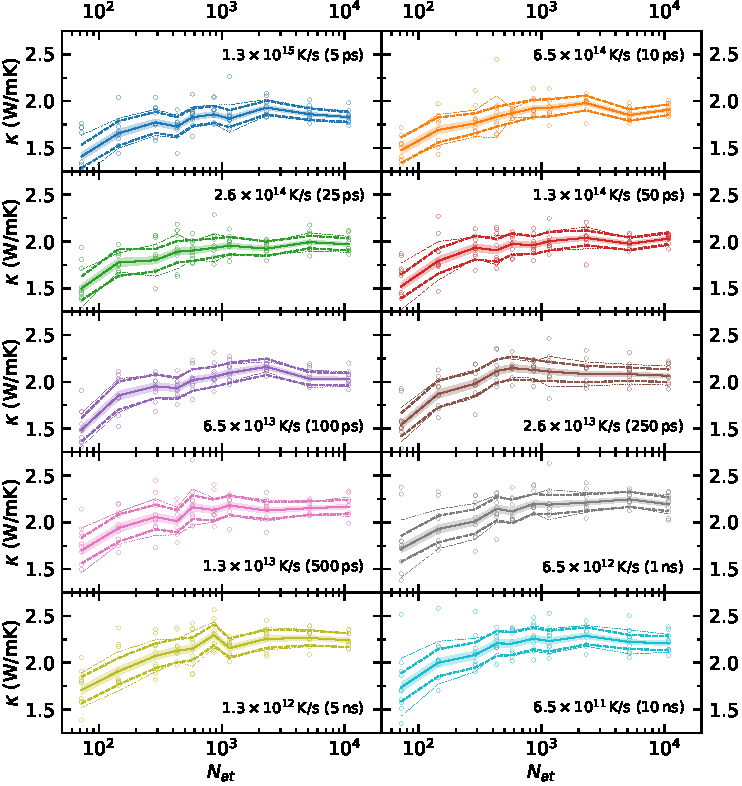
\includegraphics[width=\textwidth]{chapters/chapter6/figures/Silica_NVT_kappa_NATconv.pdf}
    \caption{Study of convergence of the thermal conductivity of a-SiO$_2$ at $500\un{K}$ with the size of the system, estimated from classical simulations, as described in Sec.~\ref{sec:results-class-quench}. 
    The abscissa indicate the number of atoms of the system, each panel corresponds to a different quenching rate $\gamma$ (the relative quenching time $t_\mathrm{quench}$ is indicated in brackets). 
    Circles are the results of $10$ independent replicas simulated with the same quenching protocol. The solid line is a weighted average computed over the replicas and weighted using the errors estimated from cepstral analysis. Three different error limits are indicated. 
    Dashed area: standard deviation of the weighted mean. 
    Dashed lines: statistical error estimated for a \emph{single} trajectory of $1\un{ns}$. 
    Dotted lines: sample standard deviation of the single values of $\kappa$. 
    }
    \label{fig:results-class-kappa-vs-size}
\end{figure}

In Fig.~\ref{fig:results-class-kappa-vs-size} we plot the thermal conductivity as a function of the number of atoms of the system $N_{at}$, for the ten quenching rates considered. 
The $\kappa$ measured for each replica is depicted with a circle. 
For each $N_{at}$ and $\gamma$, we computed a weighted average over the replicas' results (depicted with a solid line) using the errors estimated from cepstral analysis as weights. 
We can infer that $\kappa$ is underestimated by the smallest systems considered, and seems to converge to a stable value for $N_{at}\gtrsim 500$ atoms. 
This is likely due to two effects, both entering this analysis. 
One is the fact that small replicas cannot account for the whole ensemble of possible amorphous structures. In particular, the variety of medium- and long-range structures needs larger system to be correctly accounted for. However, as we mentioned in Sec.~\ref{sec:silica-size}, some authors found that averaging over a little set of small structures ($N_{at}=72$) should be enough to sufficiently reproduce the range of glass-network structures found in larger cells \cite{VanGinhoven2005}. 
Nevertheless, the smallest systems lead to an underestimate of $\kappa$ by more than $20\%$. We can probably attribute this behavior to effects on the vibrational modes: the finite-size of the system dictates an upper limit to the wavelength that can be accommodated into the simulation cell, and alters the the low and medium vibrational frequencies, which are largely attributed to the collective modes of silica. The Green-Kubo equation thus requires a sufficiently large volume to correctly account for all the contributions. 
We should however point out that this value is remarkably lower than the typical cell lengths required by NEMD calculations (\LEnote{NAT necessari in NEMD?}).

\begin{figure}[!tb]
    \centering
    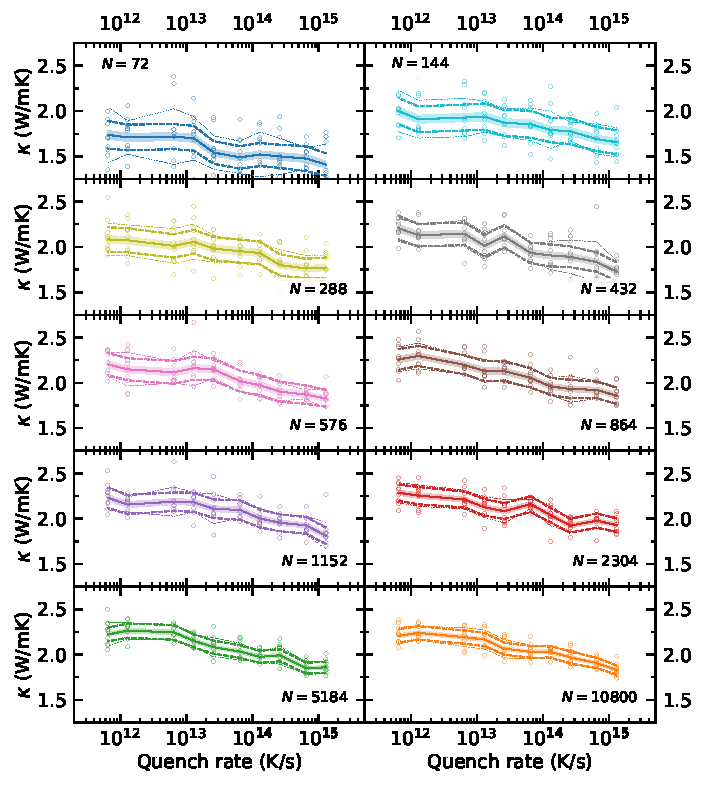
\includegraphics[width=\textwidth]{chapters/chapter6/figures/Silica_NVT_kappa_QTIMEconv.pdf}
    \caption{Study of convergence of the thermal conductivity of a-SiO$_2$ at $500\un{K}$ with the cooling quenching rate $\gamma$, estimated from classical simulations, as described in Sec.~\ref{sec:results-class-quench}. 
    Each panel corresponds to a different system sizes with $N_{at}$ atoms.
    Circles are the results of $10$ independent replicas simulated with the same quenching protocol. The solid line is a weighted average computed over the replicas and weighted using the errors estimated from cepstral analysis. Three different error limits are indicated. 
    Dashed area: standard deviation of the weighted mean. 
    Dashed lines: statistical error estimated for a \emph{single} trajectory of $1\un{ns}$. 
    Dotted lines: sample standard deviation of the single values of $\kappa$. 
    }
    \label{fig:results-class-kappa-vs-quench}
\end{figure}

In Fig.~\ref{fig:results-class-kappa-vs-quench}, the same data are plotted as a function of the quenching rate $\gamma = \frac{6500\un{K}}{t_{\mathrm{quench}}}$, for each of the sizes considered. 
Slower quenching rates (longer quenching times, of the order of a few nanoseconds) definitely lead to higher thermal conductivities. 
This is not very surprising: as we discussed in Sec.~\ref{sec:silica-quenching}, a slower quenching allows the system to relax more and to build glass structures with higher local order, less defects, and structural features that are in better agreement with experiments. 
Therefore, a quenching rate $\gamma \lesssim 10^{13}\un{K/s}$ seems to be the requirement for almost all the simulated sizes. 

In Fig.~\ref{fig:results-class-kappa-vs-size} and \ref{fig:results-class-kappa-vs-quench} the error on the weighted average is indicated as a thin shaded area surrounding the solid line. Two other lines are reported. The dashed lines delimit the average error that we expect to obtain from a single trajectory sample of $t_{\mathrm{run}}=1\un{ns}$ (it is about the error on the weighted averaged times $\sqrt{10}$). 
We observe that in general the single calculations of $\kappa$ ($10$ replicas for each abscissa, represented by single circles), fall mostly inside this error bars, for the medium and large systems. For the smaller systems, the fluctuations of the single values become bigger, probably due to larger differences in their structures, in addition to the intrinsically larger fluctuations due to the smaller size. 
The fluctuations of $\kappa$ can also be quantified by the standard deviation of $\kappa$ computed over the replicas, indicated with thin dotted lines, that becomes visibly larger than the expected error bars for the two or three smallest systems analyzed (even though this value, estimated from a very small sample, should be taken as indicative).
The trend of the relative error estimated for a $1\un{ns}$ trajectory as a function of the number of atoms is shown in Fig.~\ref{fig:results-class-kappaerror-vs-size} for $4$ selected quenching rates. The estimated relative error decreases as $\sim 1/\sqrt{N_\mathrm{nat}}$, \LEnote{suggesting that it is influenced by the fluctuations of ... the energy?? in the NVE ensemble, that decrease with the same trend.}
The quenching rate, instead, does not appear to affect the error on $\kappa$, as shown in Fig.~\ref{fig:results-class-kappaerror-vs-quench}. 

\begin{figure}[!tb]
    \centering
    \subfigure[\label{fig:results-class-kappaerror-vs-size}]{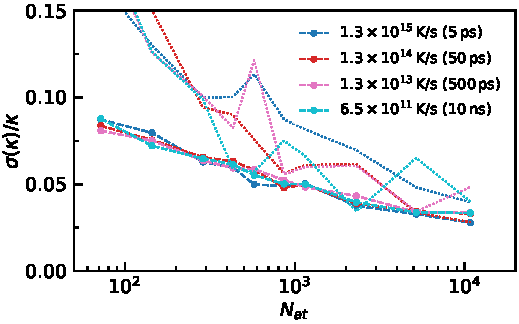
\includegraphics[width=0.49\textwidth]{chapters/chapter6/figures/silica_NVT_kappa_relerror_NAT.pdf}}
    \hfill
    \subfigure[\label{fig:results-class-kappaerror-vs-quench}]{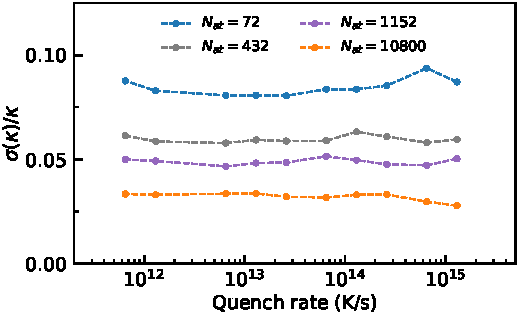
\includegraphics[width=0.49\textwidth]{chapters/chapter6/figures/silica_NVT_kappa_relerror_QTIME.pdf}}
    \caption{Thermal conductivity relative error *caption*
    Estimated relative error on the thermal conductivity of a-SiO$_2$ for a $1\un{ns}$ trajectory (dashed lines) as a function of (a) the number of atoms, (b) the cooling quenching rate. 
    Dotted lines: sample standard deviation computed over the results of $10$ replicas.
    }
    \label{fig:results-class-kappaerror}
\end{figure}

From this analysis we conclude that size of the system and cooling rate considerably affect the thermal conductivity of BKS silica glass. 
In order to perform an \abinitio study of the thermal conductivity, we need to select a sample size that can be simulated with AIMD at a reasonable computational cost. 
We decided to use one of the samples with $N_{\mathrm{nat}}=432$ atoms that were generated using the smallest cooling rate analyzed, $\gamma=6.5\times 10^{11}\un{K/s}$, corresponding to a quenching time of $10\un{ns}$. In the following we dub this sample $\S1$. 
We first made sure that $\S1$ did not exhibit any coordination defects, then we computed its thermal conductivity, that is equal to $\kappa_\S1 = ... \un{W/mK}$, using a $1\un{ns}$-long trajectory. 
This value differs from the average values obtained for the largest systems analyzed by less than $5\%$ ($\approx 0.1\un{W/mK})$. 
Further data analysis showed that an error of the order of $..\%$ could be obtained from a trajectory of $100\un{ps}$, which is a simulation length reasonably affordable with CPMD, hence making this bias in the thermal conductivity negligible. 


\LEnote{* Da inserire:\\
SAMPLE SELEZIONATO}


\subsection{Cepstral analysis}  \label{sec:results-class-cepstral}
\paragraph{Dependence on cutoff frequency $f^*$}
(For the chosen sample at experimental density)
(comparison bw normal and vel-renormalized results)

\begin{figure}[!tb]
    \centering
    \subfigure[\label{fig:csilica-sample-expdens-fstar-100ps}]{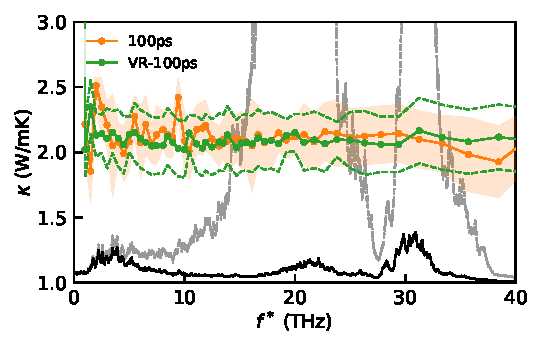
\includegraphics[width=8cm]{chapters/chapter6/figures/silica_expdens_kappa_fstar_VR_100ps.pdf}}
    \subfigure[\label{fig:csilica-sample-expdens-fstar-1ns}]{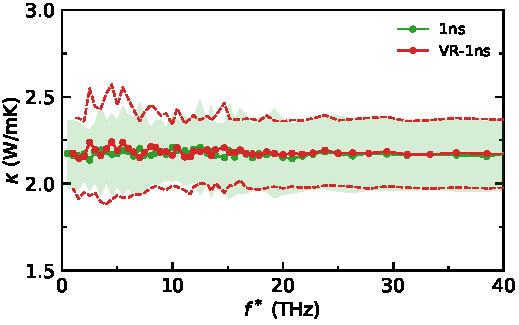
\includegraphics[width=8cm]{chapters/chapter6/figures/silica_expdens_kappa_fstar_VR_1ns.pdf}}
    \subfigure[\label{fig:csilica-sample-expdens-fstar-10ns}]{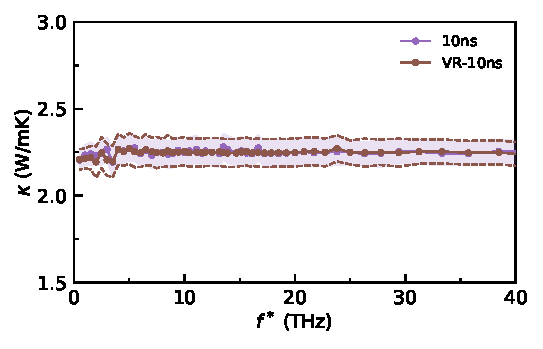
\includegraphics[width=8cm]{chapters/chapter6/figures/silica_expdens_kappa_fstar_VR_10ns.pdf}}
    \caption{Dependence of $\kappa$ on the choice of the cutoff frequency $f^*$, estimated from \emph{one} sample of (a) $100\un{ps}$, (b) $1\un{ns}$, and (c) $10\un{ps}$ of the ``original'' and VR heat flux time series. 
    The original and VR periodograms are reported for reference with grey and black lines, respectively.}
    \label{fig:csilica-sample-expdens-fstar}
\end{figure}
Fig.~\ref{fig:csilica-sample-expdens-fstar} -- stability of $\kappa$ as a function of $f^*$ increases with the length of the trajectory, as its predicted error decreases. The values and errors of $\kappa$ obtained from the VR time series are equivalent to the ones obtained from the original time series, and are slightly more stable with $f^*$. This is probably due to the much smaller power of the power spectrum of the VR heat flux, that may decrease the small artifacts introduced by the low-pass filter applied before resampling. 
Any frequency in the central region of the spectrum can be taken as $f^*$, hence we choose to set $f^*=28\un{THz}$. Conversely, a $f^*$ too small makes $\kappa$ deviate sensibly, due to the fact that the low-pass filter is not strong enough to avoid aliasing effects that modify the spectrum of the resampled time series; instead, a $f^*$ that is too high ($f^*\gtrsim 60\un{THz}$) induces a bias in $\kappa$, due to the fact the log-periodogram diverges to negative values and we start to have problems of numerical precision.



\subsection{Volume dependence}
(NEGLECTED)

\subsection{Temperature dependence}
AND THERMAL CURRENT CONTRIBUTIONS (CONV, VIR, X)


%%%%%%%%%%%%%%%%%%%%%%%%%%%%%%%%%%%%%%%%%%%%%%%%%5
\section{Quantum simulations}  \label{sec:results-quantum}
QUANTUM

\subsection{Setup}  \label{sec:results-quantum-setup}

\subsection{Heat current calculation}  \label{sec:results-quantum-current}
DT HEAT CURRENT

\subsection{Results}  \label{sec:results-quantum-results}
